% ==============================================================================
% CHAPTER 2 — Linear and Polynomial Regression
% ==============================================================================
\chapter{Linear and Polynomial Regression}\label{ch:regression}

\begin{intuition}[title=\textbf{Chapter Overview}]
Regression is the cornerstone of supervised learning: given input features $\bm{x}$, predict a continuous target $y$. This chapter builds the theory from a single variable to arbitrary polynomial complexity, derives every estimator in closed form, and introduces gradient descent as a scalable alternative.
\end{intuition}

% ------------------------------------------------------------------------------
\section{Simple Linear Regression}
% ------------------------------------------------------------------------------

\begin{definition}[Simple Linear Model]
Given a dataset $\{(x_i, y_i)\}_{i=1}^{n}$ with $x_i, y_i \in \R$, the simple linear regression model assumes
\[
    y_i = \beta_0 + \beta_1 x_i + \varepsilon_i, \qquad \varepsilon_i \overset{\text{iid}}{\sim} \mathcal{N}(0, \sigma^2).
\]
The parameters $\beta_0$ (intercept) and $\beta_1$ (slope) are unknown and must be estimated from data.
\end{definition}

\subsection{Ordinary Least Squares Derivation}

We seek $\hat{\beta}_0, \hat{\beta}_1$ that minimise the residual sum of squares:
\[
    \text{RSS}(\beta_0, \beta_1)
    = \sum_{i=1}^{n} (y_i - \beta_0 - \beta_1 x_i)^2.
\]

\begin{theorem}[OLS Estimators --- Simple Case]
Setting the partial derivatives to zero yields
\[
    \hat{\beta}_1 = \frac{\sum_{i=1}^{n}(x_i - \bar{x})(y_i - \bar{y})}{\sum_{i=1}^{n}(x_i - \bar{x})^2}
    = \frac{\widehat{\Cov}(X,Y)}{\widehat{\Var}(X)},
    \qquad
    \hat{\beta}_0 = \bar{y} - \hat{\beta}_1 \bar{x}.
\]
\end{theorem}

\begin{proof}
Taking partial derivatives of $\text{RSS}$:
\begin{align}
    \frac{\partial \text{RSS}}{\partial \beta_0}
    &= -2 \sum_{i=1}^{n}(y_i - \beta_0 - \beta_1 x_i) = 0
    \;\Longrightarrow\;
    n\beta_0 = \sum y_i - \beta_1 \sum x_i, \label{eq:ols1}\\
    \frac{\partial \text{RSS}}{\partial \beta_1}
    &= -2 \sum_{i=1}^{n} x_i(y_i - \beta_0 - \beta_1 x_i) = 0. \label{eq:ols2}
\end{align}
Substituting $\beta_0 = \bar{y} - \beta_1 \bar{x}$ from \eqref{eq:ols1} into \eqref{eq:ols2} and simplifying gives the stated formula for $\hat{\beta}_1$.
\end{proof}

\subsection{Properties of the OLS Estimators}

\begin{proposition}[Unbiasedness]
Under the model assumptions, $\E[\hat{\beta}_0] = \beta_0$ and $\E[\hat{\beta}_1] = \beta_1$.
\end{proposition}

\begin{proposition}[Variance of OLS Estimators]
\[
    \Var(\hat{\beta}_1) = \frac{\sigma^2}{\sum_{i=1}^{n}(x_i - \bar{x})^2},
    \qquad
    \Var(\hat{\beta}_0) = \sigma^2\left(\frac{1}{n} + \frac{\bar{x}^2}{\sum_{i=1}^{n}(x_i-\bar{x})^2}\right).
\]
An unbiased estimator of $\sigma^2$ is $\hat{\sigma}^2 = \frac{\text{RSS}}{n-2}$.
\end{proposition}

\begin{definition}[Coefficient of Determination]
The coefficient of determination $R^2$ measures the proportion of variance explained:
\[
    R^2 = 1 - \frac{\text{RSS}}{\text{TSS}}
    = 1 - \frac{\sum_{i=1}^{n}(y_i - \hat{y}_i)^2}{\sum_{i=1}^{n}(y_i - \bar{y})^2},
    \qquad R^2 \in [0,1].
\]
\end{definition}

\begin{remark}
In simple regression, $R^2 = r_{xy}^2$ where $r_{xy}$ is the Pearson correlation coefficient. Adding more features can only increase $R^2$ (or leave it unchanged), which motivates the \emph{adjusted} $R^2$:
\[
    R^2_{\text{adj}} = 1 - \frac{n-1}{n-p-1}(1-R^2).
\]
\end{remark}

% ------------------------------------------------------------------------------
\section{Multiple Linear Regression}
% ------------------------------------------------------------------------------

\begin{definition}[Multiple Linear Model]
With $p$ features the model becomes
\[
    \bm{y} = \bm{X}\bm{\beta} + \bm{\varepsilon},
    \qquad
    \bm{X} \in \R^{n \times (p+1)},\;
    \bm{\beta} \in \R^{p+1},\;
    \bm{\varepsilon} \sim \mathcal{N}(\bm{0}, \sigma^2 \bm{I}_n),
\]
where the first column of $\bm{X}$ is the constant $\bm{1}_n$ (intercept term).
\end{definition}

\subsection{Normal Equations}

\begin{theorem}[OLS in Matrix Form]\label{thm:normal-eq}
If $\bm{X}^\top \bm{X}$ is invertible, the unique minimiser of $\norm{\bm{y} - \bm{X}\bm{\beta}}^2$ is
\[
    \hat{\bm{\beta}} = (\bm{X}^\top \bm{X})^{-1} \bm{X}^\top \bm{y}.
\]
\end{theorem}

\begin{proof}
Define $f(\bm{\beta}) = (\bm{y}-\bm{X}\bm{\beta})^\top(\bm{y}-\bm{X}\bm{\beta})$. Expanding:
\[
    f(\bm{\beta}) = \bm{y}^\top\bm{y} - 2\bm{\beta}^\top\bm{X}^\top\bm{y} + \bm{\beta}^\top\bm{X}^\top\bm{X}\bm{\beta}.
\]
Taking the gradient and setting it to zero:
\[
    \nabla_{\bm{\beta}} f = -2\bm{X}^\top\bm{y} + 2\bm{X}^\top\bm{X}\bm{\beta} = \bm{0}
    \;\Longrightarrow\;
    \bm{X}^\top\bm{X}\bm{\beta} = \bm{X}^\top\bm{y}.
\]
Since $\bm{X}^\top\bm{X}$ is positive definite (hence invertible) when $\bm{X}$ has full column rank, we obtain the stated solution. The Hessian $2\bm{X}^\top\bm{X} \succeq 0$ confirms this is a minimum.
\end{proof}

\begin{proposition}[Gauss--Markov Theorem]
Among all linear unbiased estimators of $\bm{\beta}$, the OLS estimator $\hat{\bm{\beta}}$ has the smallest variance (in the matrix sense). That is, for any other linear unbiased estimator $\tilde{\bm{\beta}}$,
\[
    \Var(\tilde{\bm{\beta}}) - \Var(\hat{\bm{\beta}}) \succeq 0
    \quad (\text{positive semi-definite}).
\]
\end{proposition}

\begin{proposition}[Distribution of OLS Estimator]
Under the Gaussian noise assumption:
\[
    \hat{\bm{\beta}} \sim \mathcal{N}\bigl(\bm{\beta},\;\sigma^2(\bm{X}^\top\bm{X})^{-1}\bigr).
\]
This allows construction of confidence intervals and hypothesis tests. A $t$-test for $H_0: \beta_j = 0$ uses the statistic $t_j = \hat{\beta}_j / \text{se}(\hat{\beta}_j)$ with $n-p-1$ degrees of freedom.
\end{proposition}

\subsection{Geometric Interpretation}

\begin{intuition}[title=\textbf{Projection Viewpoint}]
The fitted values $\hat{\bm{y}} = \bm{X}\hat{\bm{\beta}} = \bm{H}\bm{y}$ are the orthogonal projection of $\bm{y}$ onto the column space of $\bm{X}$, where $\bm{H} = \bm{X}(\bm{X}^\top\bm{X})^{-1}\bm{X}^\top$ is the \emph{hat matrix}. The residual vector $\bm{e} = \bm{y} - \hat{\bm{y}}$ is orthogonal to every column of $\bm{X}$.
\end{intuition}

\begin{center}
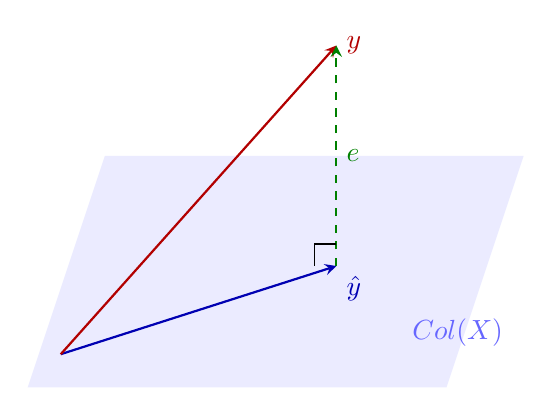
\begin{tikzpicture}[scale=1.4, >=stealth]
    % Column space plane
    \fill[blue!8] (-0.3,-0.3) -- (3.5,-0.3) -- (4.2,1.8) -- (0.4,1.8) -- cycle;
    \node[blue!60] at (3.6,0.2) {$\text{Col}(\bm{X})$};
    % Vectors
    \draw[->, thick, blue!70!black] (0,0) -- (2.5,0.8) node[below right] {$\hat{\bm{y}}$};
    \draw[->, thick, red!70!black] (0,0) -- (2.5,2.8) node[right] {$\bm{y}$};
    \draw[->, thick, green!50!black, dashed] (2.5,0.8) -- (2.5,2.8) node[midway, right] {$\bm{e}$};
    % Right angle
    \draw (2.5,1.0) -- (2.3,1.0) -- (2.3,0.8);
\end{tikzpicture}
\end{center}

% ------------------------------------------------------------------------------
\section{Polynomial Regression}
% ------------------------------------------------------------------------------

\begin{definition}[Polynomial Regression of Degree $d$]
Given scalar input $x$, the degree-$d$ polynomial model is
\[
    y = \beta_0 + \beta_1 x + \beta_2 x^2 + \cdots + \beta_d x^d + \varepsilon.
\]
This is a \emph{linear} model in the extended feature vector $\bm{\phi}(x) = (1, x, x^2, \ldots, x^d)^\top$.
\end{definition}

\begin{warning}[title=\textbf{Overfitting Risk}]
High-degree polynomials can interpolate training data perfectly while generalising poorly. The bias--variance trade-off governs model selection: low $d$ may underfit (high bias), high $d$ may overfit (high variance). Cross-validation is essential.
\end{warning}

\begin{proposition}[Bias--Variance Decomposition]
For a fixed test point $\bm{x}_0$ and squared loss, the expected prediction error decomposes as
\[
    \E\bigl[(y_0 - \hat{f}(\bm{x}_0))^2\bigr]
    = \underbrace{\Bias^2\!\bigl(\hat{f}(\bm{x}_0)\bigr)}_{\text{systematic error}}
    + \underbrace{\Var\!\bigl(\hat{f}(\bm{x}_0)\bigr)}_{\text{estimation variance}}
    + \sigma^2.
\]
\end{proposition}

\begin{proof}
Let $f_0 = f(\bm{x}_0)$ denote the true regression function. Then
\begin{align*}
    \E[(y_0 - \hat{f})^2]
    &= \E[(y_0 - f_0 + f_0 - \E[\hat{f}] + \E[\hat{f}] - \hat{f})^2]\\
    &= \E[(y_0-f_0)^2] + (f_0-\E[\hat{f}])^2 + \E[(\hat{f}-\E[\hat{f}])^2]\\
    &= \sigma^2 + \Bias^2(\hat{f}) + \Var(\hat{f}),
\end{align*}
where cross-terms vanish by independence and the fact that $\E[\hat{f}-\E[\hat{f}]]=0$.
\end{proof}

\begin{example}[Choosing Polynomial Degree]
Consider fitting $y = \sin(2\pi x) + \varepsilon$ on $[0,1]$:
\begin{itemize}
    \item $d=1$ (line): high bias, misses curvature.
    \item $d=3$: reasonable compromise, captures the shape.
    \item $d=15$: oscillates wildly between data points (Runge phenomenon).
\end{itemize}
Cross-validation typically selects $d \in \{3,4,5\}$ for this example.
\end{example}

% ------------------------------------------------------------------------------
\section{Gradient Descent}
% ------------------------------------------------------------------------------

\begin{definition}[Gradient Descent Update]
For a differentiable loss $J(\bm{\beta})$ and learning rate $\eta > 0$:
\[
    \bm{\beta}^{(t+1)} = \bm{\beta}^{(t)} - \eta\,\nabla J(\bm{\beta}^{(t)}).
\]
\end{definition}

\begin{algorithme}[title=\textbf{Batch Gradient Descent for Linear Regression}]
\begin{enumerate}
    \item Initialise $\bm{\beta}^{(0)}$ (e.g.\ zeros).
    \item At each iteration $t$, compute
    \[
        \nabla J = \frac{2}{n}\bm{X}^\top(\bm{X}\bm{\beta}^{(t)} - \bm{y}).
    \]
    \item Update: $\bm{\beta}^{(t+1)} \leftarrow \bm{\beta}^{(t)} - \eta\,\nabla J$.
    \item Repeat until $\norm{\nabla J} < \epsilon$ or maximum iterations reached.
\end{enumerate}
\end{algorithme}

\begin{theorem}[Convergence of Gradient Descent]
If $J$ is $L$-smooth and convex, gradient descent with step size $\eta = 1/L$ satisfies
\[
    J(\bm{\beta}^{(t)}) - J(\bm{\beta}^*) \leq \frac{L\norm{\bm{\beta}^{(0)} - \bm{\beta}^*}^2}{2t}.
\]
For linear regression, the smoothness constant is $L = \frac{2}{n}\lambda_{\max}(\bm{X}^\top\bm{X})$.
\end{theorem}

\begin{definition}[Stochastic Gradient Descent]
At each iteration, pick a random index $i_t \in \{1,\ldots,n\}$ and update
\[
    \bm{\beta}^{(t+1)} = \bm{\beta}^{(t)} - \eta_t\,\nabla J_{i_t}(\bm{\beta}^{(t)}),
    \qquad \nabla J_i = 2((\bm{x}_i^\top\bm{\beta}^{(t)}) - y_i)\bm{x}_i.
\]
Each step costs $O(p)$ instead of $O(np)$, but introduces variance in the gradient estimate.
\end{definition}

\begin{bestpractice}[title=\textbf{Stochastic and Mini-Batch Variants}]
\textbf{SGD:} Replace the full gradient with a single-sample estimate $\nabla J_i$. Convergence is noisier but each step costs $O(p)$ instead of $O(np)$. Use a decaying learning rate $\eta_t = \eta_0 / t$.\\[3pt]
\textbf{Mini-batch:} Use a random subset of size $B$. A good default is $B \in \{32, 64, 128\}$. This balances the speed of SGD with the stability of batch GD.
\end{bestpractice}

% ------------------------------------------------------------------------------
\section{Implementation in Python}
% ------------------------------------------------------------------------------

\subsection{From Scratch}

\begin{codeblock}[title=\textbf{OLS from Scratch}]
\begin{minted}{python}
import numpy as np

def ols_fit(X, y):
    """Ordinary least squares via the normal equations."""
    # Add intercept column
    ones = np.ones((X.shape[0], 1))
    X_aug = np.hstack([ones, X])
    # Normal equations: beta = (X^T X)^{-1} X^T y
    beta = np.linalg.solve(X_aug.T @ X_aug, X_aug.T @ y)
    return beta

def ols_predict(X, beta):
    ones = np.ones((X.shape[0], 1))
    X_aug = np.hstack([ones, X])
    return X_aug @ beta

# Generate synthetic data
np.random.seed(42)
X = 2 * np.random.rand(100, 1)
y = 4 + 3 * X.ravel() + np.random.randn(100)

beta = ols_fit(X, y)
print(f"Intercept: {beta[0]:.3f}, Slope: {beta[1]:.3f}")
\end{minted}
\end{codeblock}

\begin{codeoutput}
\begin{minted}{text}
Intercept: 4.215, Slope: 2.770
\end{minted}
\end{codeoutput}

\subsection{Gradient Descent from Scratch}

\begin{codeblock}[title=\textbf{Gradient Descent Implementation}]
\begin{minted}{python}
def gradient_descent(X, y, eta=0.1, n_iter=1000):
    ones = np.ones((X.shape[0], 1))
    X_aug = np.hstack([ones, X])
    n, p = X_aug.shape
    beta = np.zeros(p)
    losses = []
    for t in range(n_iter):
        residuals = X_aug @ beta - y
        grad = (2 / n) * X_aug.T @ residuals
        beta -= eta * grad
        losses.append(np.mean(residuals**2))
    return beta, losses

beta_gd, loss_history = gradient_descent(X, y, eta=0.05, n_iter=2000)
print(f"GD Intercept: {beta_gd[0]:.3f}, GD Slope: {beta_gd[1]:.3f}")
print(f"Final MSE: {loss_history[-1]:.4f}")
\end{minted}
\end{codeblock}

\begin{codeoutput}
\begin{minted}{text}
GD Intercept: 4.215, GD Slope: 2.770
Final MSE: 0.9225
\end{minted}
\end{codeoutput}

\subsection{Using Scikit-Learn}

\begin{codeblock}[title=\textbf{Linear and Polynomial Regression with scikit-learn}]
\begin{minted}{python}
from sklearn.linear_model import LinearRegression
from sklearn.preprocessing import PolynomialFeatures
from sklearn.pipeline import make_pipeline
from sklearn.model_selection import cross_val_score
from sklearn.metrics import mean_squared_error, r2_score

# Simple linear regression
model = LinearRegression()
model.fit(X, y)
print(f"sklearn Intercept: {model.intercept_:.3f}")
print(f"sklearn Slope:     {model.coef_[0]:.3f}")
print(f"R^2:               {model.score(X, y):.4f}")

# Polynomial regression (degree 3)
poly_model = make_pipeline(
    PolynomialFeatures(degree=3, include_bias=False),
    LinearRegression()
)
poly_model.fit(X, y)
y_pred = poly_model.predict(X)
print(f"Poly3 MSE: {mean_squared_error(y, y_pred):.4f}")
print(f"Poly3 R^2: {r2_score(y, y_pred):.4f}")

# Cross-validation to select degree
for d in [1, 2, 3, 5, 10]:
    pipe = make_pipeline(
        PolynomialFeatures(degree=d, include_bias=False),
        LinearRegression()
    )
    cv_mse = -cross_val_score(pipe, X, y,
                               scoring="neg_mean_squared_error", cv=5)
    print(f"Degree {d:2d}: CV MSE = {cv_mse.mean():.4f} "
          f"(+/- {cv_mse.std():.4f})")
\end{minted}
\end{codeblock}

\begin{codeoutput}
\begin{minted}{text}
sklearn Intercept: 4.215
sklearn Slope:     2.770
R^2:               0.8901
Poly3 MSE: 0.9102
Poly3 R^2: 0.8932
Degree  1: CV MSE = 1.0243 (+/- 0.2148)
Degree  2: CV MSE = 1.0067 (+/- 0.2314)
Degree  3: CV MSE = 1.0401 (+/- 0.2589)
Degree  5: CV MSE = 1.2315 (+/- 0.4012)
Degree 10: CV MSE = 5.8934 (+/- 8.1247)
\end{minted}
\end{codeoutput}

% ------------------------------------------------------------------------------
\section{Regression Diagram}
% ------------------------------------------------------------------------------

\begin{center}
\begin{tikzpicture}[scale=0.9]
    % Scatter points
    \foreach \x/\y in {0.5/4.8, 1.0/6.5, 1.5/8.2, 2.0/9.0, 2.5/11.5,
                        3.0/12.8, 3.5/14.0, 4.0/15.2, 4.5/17.0, 5.0/18.5}{
        \fill[blue!70] (\x, \y*0.35) circle (2pt);
    }
    % Regression line
    \draw[red, thick] (0.2, 1.5) -- (5.3, 6.7);
    % Residuals
    \foreach \x/\y/\yhat in {1.0/6.5/5.1, 2.5/11.5/9.6, 4.0/15.2/14.1}{
        \draw[green!50!black, dashed, thin] (\x, \y*0.35) -- (\x, \yhat*0.35);
    }
    % Axes
    \draw[->] (0,0) -- (5.8,0) node[right] {$x$};
    \draw[->] (0,0) -- (0,7.5) node[above] {$y$};
    \node[red] at (4.5,7.2) {$\hat{y} = \hat{\beta}_0 + \hat{\beta}_1 x$};
    \node[green!50!black] at (4.0,4.2) {residuals};
\end{tikzpicture}
\end{center}

% ------------------------------------------------------------------------------
\section{Assumptions and Diagnostics}
% ------------------------------------------------------------------------------

\begin{definition}[Assumptions of Linear Regression]
The classical linear model relies on four key assumptions:
\begin{enumerate}
    \item \textbf{Linearity:} $\E[y|\bm{x}] = \bm{x}^\top\bm{\beta}$.
    \item \textbf{Independence:} the errors $\varepsilon_i$ are mutually independent.
    \item \textbf{Homoscedasticity:} $\Var(\varepsilon_i) = \sigma^2$ for all $i$.
    \item \textbf{Normality:} $\varepsilon_i \sim \mathcal{N}(0,\sigma^2)$ (needed for exact inference, not for OLS consistency).
\end{enumerate}
\end{definition}

\begin{bestpractice}[title=\textbf{Diagnostic Plots}]
\begin{itemize}
    \item \textbf{Residuals vs.\ fitted:} should show no pattern. A funnel shape indicates heteroscedasticity.
    \item \textbf{Q--Q plot:} residuals should lie on the $45°$ line if normality holds.
    \item \textbf{Scale-location:} $\sqrt{|\text{standardised residuals}|}$ vs.\ fitted values checks for non-constant variance.
    \item \textbf{Leverage plot:} identifies influential observations via hat values $h_{ii}$ and Cook's distance $D_i$.
\end{itemize}
\end{bestpractice}

\begin{definition}[Cook's Distance]
Cook's distance for observation $i$ measures its influence on the fitted values:
\[
    D_i = \frac{(\hat{\bm{y}} - \hat{\bm{y}}_{(i)})^\top(\hat{\bm{y}} - \hat{\bm{y}}_{(i)})}{(p+1)\hat{\sigma}^2}
    = \frac{e_i^2}{(p+1)\hat{\sigma}^2}\cdot\frac{h_{ii}}{(1-h_{ii})^2},
\]
where $\hat{\bm{y}}_{(i)}$ denotes predictions when observation $i$ is removed. Points with $D_i > 1$ (or $D_i > 4/n$) deserve closer inspection.
\end{definition}

% ------------------------------------------------------------------------------
\section{Exercises}
% ------------------------------------------------------------------------------

\begin{exercise}[Derivation]
Starting from the RSS for simple linear regression, verify the second-order conditions: show that the Hessian matrix is positive definite, confirming that the OLS solution is indeed a minimum.
\end{exercise}

\begin{exercise}[Normal Equations Complexity]
Show that solving the normal equations $\bm{X}^\top\bm{X}\bm{\beta} = \bm{X}^\top\bm{y}$ via Cholesky decomposition costs $O(np^2 + p^3/3)$. When is gradient descent preferable?
\end{exercise}

\begin{exercise}[Polynomial Overfitting]
Generate $n=30$ points from $y = \sin(2\pi x) + \varepsilon$ with $x \sim \mathcal{U}(0,1)$ and $\varepsilon \sim \mathcal{N}(0,0.2)$.
\begin{enumerate}
    \item Fit polynomials of degrees $d \in \{1, 3, 5, 10, 20\}$.
    \item Plot training and test MSE as a function of $d$.
    \item Identify the best degree using 5-fold cross-validation.
\end{enumerate}
\end{exercise}

\begin{exercise}[Gradient Descent Convergence]
Implement gradient descent for linear regression. Experiment with learning rates $\eta \in \{0.001, 0.01, 0.1, 1.0\}$ and plot the loss curve $J(\bm{\beta}^{(t)})$ versus iteration $t$. Explain what happens when $\eta$ is too large.
\end{exercise}

\begin{exercise}[Hat Matrix Properties]
Prove the following properties of the hat matrix $\bm{H} = \bm{X}(\bm{X}^\top\bm{X})^{-1}\bm{X}^\top$:
\begin{enumerate}
    \item $\bm{H}$ is symmetric and idempotent ($\bm{H}^2 = \bm{H}$).
    \item $\text{tr}(\bm{H}) = p + 1$.
    \item $(\bm{I} - \bm{H})\bm{X} = \bm{0}$.
    \item The eigenvalues of $\bm{H}$ are either $0$ or $1$.
\end{enumerate}
\end{exercise}

\begin{exercise}[Multi-Feature Regression]
Load the \texttt{diabetes} dataset from \texttt{sklearn.datasets}. Fit a multiple linear regression, report $R^2$ on an 80/20 train/test split, and interpret the three largest coefficients. Compute the adjusted $R^2$ and compare.
\end{exercise}

\begin{exercise}[Comparing Normal Equations and GD]
On the \texttt{diabetes} dataset, compare the coefficients obtained via the normal equations (\texttt{np.linalg.solve}) with those from gradient descent (1000 iterations, $\eta=0.01$). Plot $\norm{\bm{\beta}^{(t)} - \hat{\bm{\beta}}_{\text{OLS}}}$ vs.\ $t$. How many iterations are needed to achieve $<10^{-6}$ error?
\end{exercise}

\begin{keyformulas}[title=\textbf{Chapter 2 Summary}]
\begin{itemize}
    \item \textbf{Simple OLS:} $\hat{\beta}_1 = \frac{\widehat{\Cov}(X,Y)}{\widehat{\Var}(X)},\quad \hat{\beta}_0 = \bar{y} - \hat{\beta}_1\bar{x}$
    \item \textbf{Multiple OLS:} $\hat{\bm{\beta}} = (\bm{X}^\top\bm{X})^{-1}\bm{X}^\top\bm{y}$
    \item \textbf{Gradient Descent:} $\bm{\beta}^{(t+1)} = \bm{\beta}^{(t)} - \frac{2\eta}{n}\bm{X}^\top(\bm{X}\bm{\beta}^{(t)} - \bm{y})$
    \item \textbf{Polynomial:} Linear in $\bm{\phi}(x) = (1, x, \ldots, x^d)^\top$
    \item \textbf{Bias--Variance:} $\E[(y-\hat{f})^2] = \Bias^2 + \Var + \sigma^2$
    \item \textbf{$R^2$:} $1 - \text{RSS}/\text{TSS}$, \quad $R^2_{\text{adj}} = 1 - \frac{n-1}{n-p-1}(1-R^2)$
\end{itemize}
\end{keyformulas}
